% f2015zjl_q13_tetra.tex — 2015 年高考数学·浙江卷·理科 第 13 题（三棱锥与两中点）
%
% 【来源】`.work/phase3-b19/source/2015浙江理.pdf`（SHA-256
%   801150f0a6d440ac967813d264face6d48b6ee9c69cc20f1c9d6b2b38dec2e9f），
%   第 1 页（合订本页 989）；内容对象 5。逐路径实测见
%   `.work/phase3-b19/figure-inventory.md`。
%
% 【坐标口径】源 PDF 用户空间（原点左下、y 向上）。本图本地坐标
%   (x, y) = (x_page − 918.392, y_page − 615.313)，1 单位 = 1 TeX pt。
%   路径坐标逐点照录内容流（含三次贝塞尔控制点）。
%
% 元素计数：7 条路径（棱 AB/AC/AD/BC/CD 实线、BD 虚线、中线 AN/CM）＋6 个标签
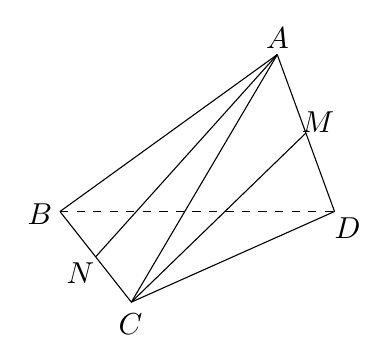
\begin{tikzpicture}[x=1pt, y=1pt,
    every node/.style={inner sep=0pt, font=\fontsize{10.5pt}{12.6pt}\selectfont}]
  \draw[line width=0.398pt] (99.2138,32.7410)   -- (78.5208,89.4350);
  \draw[line width=0.398pt] (0.0000,32.7410)   -- (25.7960,0.0000)   -- (99.2140,32.7410);
  \draw[line width=0.398pt] (78.5206,89.4346)   -- (-0.0004,32.7406);
  \draw[line width=0.398pt] (78.5206,89.4346)   -- (12.8976,16.3706);
  \draw[line width=0.398pt] (25.7957,0.0005)   -- (88.8677,61.0875);
  \draw[line width=0.398pt] (78.5206,89.4346)   -- (25.7956,0.0006);
  \draw[line width=0.398pt, dash pattern=on 2.989pt off 2.989pt, dash phase=0.0pt] (0.0000,32.7410)   -- (99.2140,32.7410);

  \node[anchor=center] at (78.558,95.427) {$A$};  % 源中心 (996.95,710.74)
  \node[anchor=center] at (93.208,65.027) {$M$};  % 源中心 (1011.60,680.34)
  \node[anchor=center] at (-7.242,31.777) {$B$};  % 源中心 (911.15,647.09)
  \node[anchor=center] at (103.958,26.827) {$D$};  % 源中心 (1022.35,642.14)
  \node[anchor=center] at (7.408,10.477) {$N$};  % 源中心 (925.80,625.79)
  \node[anchor=center] at (25.458,-7.973) {$C$};  % 源中心 (943.85,607.34)

\end{tikzpicture}
%
% 【自验结果】
%   探针：latexmk -pdfxe（待跑）。
